% Options for packages loaded elsewhere
% Options for packages loaded elsewhere
\PassOptionsToPackage{unicode}{hyperref}
\PassOptionsToPackage{hyphens}{url}
%
\documentclass[
  ignorenonframetext,
  aspectratio=169,
]{beamer}
\newif\ifbibliography
\usepackage{pgfpages}
\setbeamertemplate{caption}[numbered]
\setbeamertemplate{caption label separator}{: }
\setbeamercolor{caption name}{fg=normal text.fg}
\beamertemplatenavigationsymbolsempty
% remove section numbering
\setbeamertemplate{part page}{
  \centering
  \begin{beamercolorbox}[sep=16pt,center]{part title}
    \usebeamerfont{part title}\insertpart\par
  \end{beamercolorbox}
}
\setbeamertemplate{section page}{
  \centering
  \begin{beamercolorbox}[sep=12pt,center]{section title}
    \usebeamerfont{section title}\insertsection\par
  \end{beamercolorbox}
}
\setbeamertemplate{subsection page}{
  \centering
  \begin{beamercolorbox}[sep=8pt,center]{subsection title}
    \usebeamerfont{subsection title}\insertsubsection\par
  \end{beamercolorbox}
}
% Prevent slide breaks in the middle of a paragraph
\widowpenalties 1 10000
\raggedbottom
\usepackage{iftex}
\ifPDFTeX
  \usepackage[T1]{fontenc}
  \usepackage[utf8]{inputenc}
  \usepackage{textcomp} % provide euro and other symbols
\else % if luatex or xetex
  \usepackage{unicode-math} % this also loads fontspec
  \defaultfontfeatures{Scale=MatchLowercase}
  \defaultfontfeatures[\rmfamily]{Ligatures=TeX,Scale=1}
\fi
\usepackage{lmodern}

\usetheme[]{metropolis}
\ifPDFTeX\else
  % xetex/luatex font selection
\fi
% Use upquote if available, for straight quotes in verbatim environments
\IfFileExists{upquote.sty}{\usepackage{upquote}}{}
\IfFileExists{microtype.sty}{% use microtype if available
  \usepackage[]{microtype}
  \UseMicrotypeSet[protrusion]{basicmath} % disable protrusion for tt fonts
}{}
\makeatletter
\@ifundefined{KOMAClassName}{% if non-KOMA class
  \IfFileExists{parskip.sty}{%
    \usepackage{parskip}
  }{% else
    \setlength{\parindent}{0pt}
    \setlength{\parskip}{6pt plus 2pt minus 1pt}}
}{% if KOMA class
  \KOMAoptions{parskip=half}}
\makeatother


\usepackage{longtable,booktabs,array}
\usepackage{calc} % for calculating minipage widths
\usepackage{caption}
% Make caption package work with longtable
\makeatletter
\def\fnum@table{\tablename~\thetable}
\makeatother
\usepackage{graphicx}
\makeatletter
\newsavebox\pandoc@box
\newcommand*\pandocbounded[1]{% scales image to fit in text height/width
  \sbox\pandoc@box{#1}%
  \Gscale@div\@tempa{\textheight}{\dimexpr\ht\pandoc@box+\dp\pandoc@box\relax}%
  \Gscale@div\@tempb{\linewidth}{\wd\pandoc@box}%
  \ifdim\@tempb\p@<\@tempa\p@\let\@tempa\@tempb\fi% select the smaller of both
  \ifdim\@tempa\p@<\p@\scalebox{\@tempa}{\usebox\pandoc@box}%
  \else\usebox{\pandoc@box}%
  \fi%
}
% Set default figure placement to htbp
\def\fps@figure{htbp}
\makeatother





\setlength{\emergencystretch}{3em} % prevent overfull lines

\providecommand{\tightlist}{%
  \setlength{\itemsep}{0pt}\setlength{\parskip}{0pt}}



 


% ============================================================
%  Econ 2203 — Beamer Metropolis Theme Preamble
%  Course: International Trade and Policy in Agriculture
%  Instructor: Nithin M, Department of Development Economics
% ============================================================

% MUST be first: load Metropolis theme before \metroset and colour overrides
\usetheme{metropolis}

% Only load packages not already provided by pandoc's beamer template
\usepackage{amsmath,amssymb}

% ---- Brand colours -----------------------------------------
\definecolor{brandblue}{HTML}{012169}
\definecolor{brandgold}{HTML}{B9975B}
\definecolor{lightblue}{HTML}{E8EDF5}

% ---- Metropolis colour overrides ---------------------------
% Main palette
\setbeamercolor{normal text}{fg=black,bg=white}
\setbeamercolor{alerted text}{fg=brandgold}
\setbeamercolor{example text}{fg=brandblue!70!black}

% Title slide
\setbeamercolor{title}{fg=white,bg=brandblue}
\setbeamercolor{subtitle}{fg=brandgold}
\setbeamercolor{author}{fg=white}
\setbeamercolor{institute}{fg=brandgold!80!white}
\setbeamercolor{date}{fg=white}
\setbeamercolor{title page header}{fg=white,bg=brandblue}

% Frametitle bar
\setbeamercolor{frametitle}{fg=white,bg=brandblue}

% Progress bar → gold
\setbeamercolor{progress bar}{fg=brandgold,bg=brandblue!30}
\setbeamercolor{title separator}{fg=brandgold}
\setbeamercolor{progress bar in head/foot}{fg=brandgold,bg=brandblue!20}
\setbeamercolor{progress bar in section page}{fg=brandgold,bg=brandblue!20}

% Blocks
\setbeamercolor{block title}{bg=brandblue,fg=white}
\setbeamercolor{block body}{bg=lightblue,fg=black}
\setbeamercolor{block title alerted}{bg=brandgold,fg=white}
\setbeamercolor{block body alerted}{bg=brandgold!12,fg=black}
\setbeamercolor{block title example}{bg=brandblue!70!black,fg=white}
\setbeamercolor{block body example}{bg=brandblue!8,fg=black}

% Structure / lists
\setbeamercolor{structure}{fg=brandblue}
\setbeamercolor{section in toc}{fg=brandblue}
\setbeamercolor{itemize item}{fg=brandblue}
\setbeamercolor{itemize subitem}{fg=brandgold}
\setbeamercolor{enumerate item}{fg=brandblue}
\setbeamercolor{description item}{fg=brandblue}

% ---- Metropolis options ------------------------------------
\metroset{
  progressbar    = frametitle,   % gold bar under frametitle
  sectionpage    = none,
  numbering      = fraction,
  block          = fill
}

% ---- Fonts (Metropolis uses Fira Sans; fallback gracefully) -
\setbeamerfont{title}{size=\Large,series=\bfseries}
\setbeamerfont{subtitle}{size=\normalsize,series=\mdseries}
\setbeamerfont{frametitle}{size=\large,series=\bfseries}
\setbeamerfont{block title}{size=\normalsize,series=\bfseries}
\setbeamerfont{caption}{size=\footnotesize}

% ---- Footer: course info + slide number --------------------
\setbeamertemplate{footline}{%
  \begin{beamercolorbox}[wd=\paperwidth,ht=2.0ex,dp=1ex]{footline}%
    \hspace{0.8em}%
    {\footnotesize\color{brandblue!60}%
      Econ 2203 \textbar{} International Trade and Policy in Agriculture
      \hfill Nithin M \hfill
      \insertframenumber{}/\inserttotalframenumber\hspace{0.8em}}%
  \end{beamercolorbox}%
}

% ---- Misc --------------------------------------------------
\setlength{\parskip}{0.25em}
\setbeamertemplate{navigation symbols}{}

% tighter column sep for side-by-side content
\setlength{\columnsep}{0.8em}

% Fix: make \label truly robust in moving arguments (Quarto generates
% \caption{\label{fig-xxx}...} which crashes Metropolis in batchmode).
% DeclareRobustCommand creates a self-protecting robust version.
\makeatletter
\let\quarto@originallabel\label
\DeclareRobustCommand*{\label}[1]{\quarto@originallabel{#1}}
\makeatother

% Prevent figures from overflowing Beamer frames.
% width=\linewidth: scale to text width (already Quarto default);
% height=0.6\textheight: cap height so figures never push past the frame bottom.
% keepaspectratio: never distort — whichever constraint binds first wins.
\setkeys{Gin}{width=\linewidth,height=0.6\textheight,keepaspectratio}
\makeatletter
\@ifpackageloaded{caption}{}{\usepackage{caption}}
\AtBeginDocument{%
\ifdefined\contentsname
  \renewcommand*\contentsname{Table of contents}
\else
  \newcommand\contentsname{Table of contents}
\fi
\ifdefined\listfigurename
  \renewcommand*\listfigurename{List of Figures}
\else
  \newcommand\listfigurename{List of Figures}
\fi
\ifdefined\listtablename
  \renewcommand*\listtablename{List of Tables}
\else
  \newcommand\listtablename{List of Tables}
\fi
\ifdefined\figurename
  \renewcommand*\figurename{Figure}
\else
  \newcommand\figurename{Figure}
\fi
\ifdefined\tablename
  \renewcommand*\tablename{Table}
\else
  \newcommand\tablename{Table}
\fi
}
\@ifpackageloaded{float}{}{\usepackage{float}}
\floatstyle{ruled}
\@ifundefined{c@chapter}{\newfloat{codelisting}{h}{lop}}{\newfloat{codelisting}{h}{lop}[chapter]}
\floatname{codelisting}{Listing}
\newcommand*\listoflistings{\listof{codelisting}{List of Listings}}
\makeatother
\makeatletter
\makeatother
\makeatletter
\@ifpackageloaded{caption}{}{\usepackage{caption}}
\@ifpackageloaded{subcaption}{}{\usepackage{subcaption}}
\makeatother

\usepackage{bookmark}
\IfFileExists{xurl.sty}{\usepackage{xurl}}{} % add URL line breaks if available
\urlstyle{same}
\hypersetup{
  pdftitle={Features of International Trade},
  pdfauthor={Nithin M},
  hidelinks,
  pdfcreator={LaTeX via pandoc}}


\title{Features of International Trade}
\subtitle{Econ 2203 \textbar{} International Trade and Policy in
Agriculture}
\author{Nithin M}
\date{2026-05-02}
\institute{Department of Development Economics}

\begin{document}
\frame{\titlepage}


\section{Part I: Recap and Overview}\label{part-i-recap-and-overview}

\begin{frame}{Recap: Lecture 1}
\phantomsection\label{recap-lecture-1}
\textbf{Three things to remember from last week}

\begin{enumerate}
\item
  \textbf{International trade} = cross-border exchange of goods,
  services, and capital; driven by differences in resource endowments,
  technology, and opportunity costs
\item
  \textbf{India's position:} 18th-largest merchandise exporter;
  agricultural exports \textasciitilde\$43.7B (FY2024); structural trade
  surplus in agriculture of \textasciitilde\$15.5B
\item
  \textbf{Agricultural trade is special} --- food security concerns,
  perishability, seasonality, and powerful political economy shape how
  governments intervene
\end{enumerate}

\textbf{Today's agenda}

\begin{itemize}
\tightlist
\item
  What distinguishes international trade from \emph{domestic} trade?
\item
  How open is India to global trade --- and how has this changed over
  time?
\item
  Advantages and risks of participating in global markets
\end{itemize}
\end{frame}

\begin{frame}{India's Growing Trade Openness}
\phantomsection\label{indias-growing-trade-openness}
\begin{figure}

\centering{

\pandocbounded{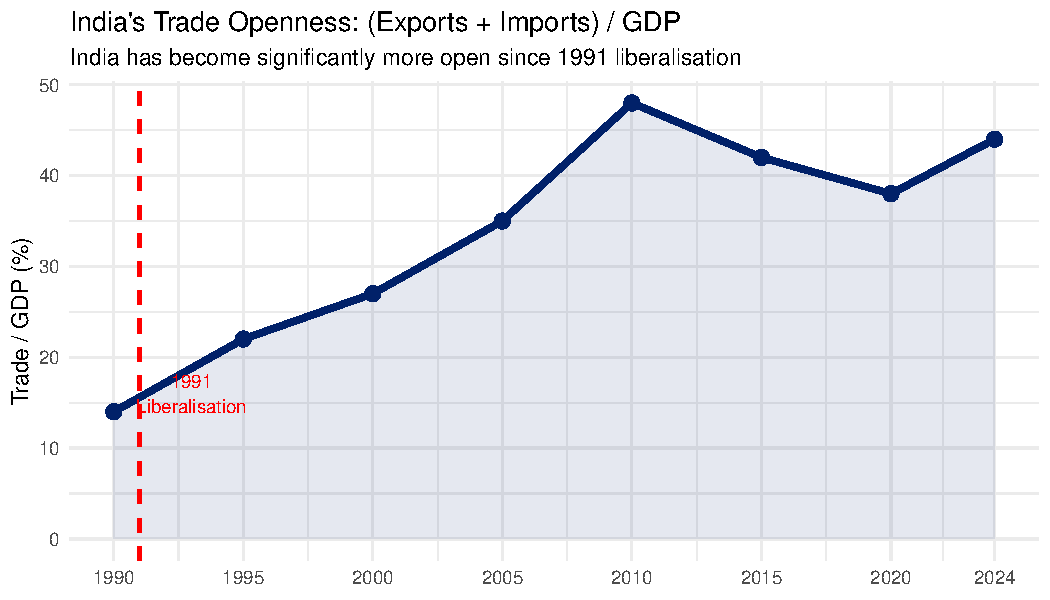
\includegraphics[keepaspectratio]{Lecture02_Features_files/figure-beamer/fig-trade-gdp-1.pdf}}

}

\caption{\label{fig-trade-gdp}India: Trade Openness (Exports + Imports
as \% of GDP) Source: World Bank, World Development Indicators (WDI).}

\end{figure}%

Trade/GDP rose from \textbf{14\% (1990)} to \textbf{44\% (2024)} ---
India is significantly more integrated into the global economy
post-liberalisation.
\end{frame}

\section{Part II: Six Key Features}\label{part-ii-six-key-features}

\begin{frame}{Features That Make International Trade Distinct}
\phantomsection\label{features-that-make-international-trade-distinct}
International trade is not simply domestic trade ``at a larger scale.''
Six features create unique challenges:

\textbf{(a) Geographical separation} --- Long distances → higher
transport costs, insurance, cold-chain requirements, longer lead times

\textbf{(b) Different currencies} --- Each transaction requires currency
conversion; exchange rate fluctuations create financial risk

\textbf{(c) Factor immobility} --- Labour and capital cannot move freely
across borders --- immigration controls, capital account restrictions

\textbf{(d) Multiple political jurisdictions} --- Each country sets its
own trade policy --- tariffs, quotas, export bans; no single governing
authority

\textbf{(e) Different legal systems \& culture} --- Food labelling laws,
packaging standards, contract enforcement vary widely

\note{\textbf{(f) Greater risk and uncertainty} --- Combination of all
above → higher commercial, political, and exchange-rate risk than
domestic commerce. Indian spice exporters must comply with EU pesticide
MRL standards.}
\end{frame}

\begin{frame}{Feature 1: Factor Immobility}
\phantomsection\label{feature-1-factor-immobility}
\textbf{Why factors don't move freely}

\begin{itemize}
\tightlist
\item
  \textbf{Labour:} Visa restrictions, language barriers, immigration
  quotas

  \begin{itemize}
  \tightlist
  \item
    India sends \textasciitilde8 million workers to Gulf countries ---
    under strict bilateral agreements, not free movement
  \end{itemize}
\item
  \textbf{Capital:} FDI restrictions, capital account controls,
  regulatory hurdles

  \begin{itemize}
  \tightlist
  \item
    India maintains partial capital account convertibility
    (RBI-regulated)
  \end{itemize}
\item
  \textbf{Land:} Completely immobile by definition
\end{itemize}

\textbf{Why this matters for trade theory}

\begin{itemize}
\tightlist
\item
  Classical models (Ricardo, H-O) assume \emph{factor immobility} across
  borders
\item
  This is what makes trade in goods a \emph{substitute} for factor flows
\item
  If labour moved freely, there would be less need to trade goods
\end{itemize}

\textbf{India case: Gulf remittances} --- Indian workers (largely from
Kerala, UP, Bihar) work in UAE, Saudi Arabia, Kuwait --- sending back
\textbf{\textasciitilde\$120 billion in remittances (FY2024)}, making
India the world's largest remittance recipient.
\end{frame}

\begin{frame}{Feature 2: Currency and Exchange Risk}
\phantomsection\label{feature-2-currency-and-exchange-risk}
\textbf{The exchange rate problem}

\begin{itemize}
\tightlist
\item
  Indian exporters price in \textbf{USD} (world standard for
  commodities)
\item
  Their costs are in \textbf{Indian Rupees (INR)}
\item
  If INR appreciates (e.g., ₹80 → ₹75 per USD), the same USD revenue
  converts to \emph{fewer rupees} → profit squeezed
\item
  If INR depreciates (₹80 → ₹85), exporters gain; importers lose
\end{itemize}

\begin{longtable}[]{@{}lllll@{}}
\toprule\noalign{}
Year & INR/USD & & Year & INR/USD \\
\midrule\noalign{}
\endhead
2000 & 45 & & 2020 & 75 \\
2010 & 46 & & 2024 & 83--84 \\
2015 & 65 & & & \\
\bottomrule\noalign{}
\end{longtable}

\textbf{Agricultural export example:} A Punjab wheat exporter quotes
\textbf{\$250/tonne} FOB Mumbai. At ₹80/USD → realises ₹20,000/tonne; at
₹75/USD → only ₹18,750/tonne. A \textbf{5\% INR appreciation = 6.25\%
reduction} in rupee revenue --- potentially wiping out margins.
\textbf{Hedging tools:} Forward contracts, futures on NSE/BSE, ECGC
insurance.
\end{frame}

\section{Part III: Internal vs International
Trade}\label{part-iii-internal-vs-international-trade}

\begin{frame}{Internal vs International Trade: Key Differences}
\phantomsection\label{internal-vs-international-trade-key-differences}
\begin{longtable}[]{@{}
  >{\raggedright\arraybackslash}p{(\linewidth - 4\tabcolsep) * \real{0.1897}}
  >{\raggedright\arraybackslash}p{(\linewidth - 4\tabcolsep) * \real{0.4483}}
  >{\raggedright\arraybackslash}p{(\linewidth - 4\tabcolsep) * \real{0.3621}}@{}}
\toprule\noalign{}
\begin{minipage}[b]{\linewidth}\raggedright
Dimension
\end{minipage} & \begin{minipage}[b]{\linewidth}\raggedright
Internal (Domestic) Trade
\end{minipage} & \begin{minipage}[b]{\linewidth}\raggedright
International Trade
\end{minipage} \\
\midrule\noalign{}
\endhead
\textbf{Factor mobility} & Labour and capital move freely & Highly
restricted --- visas, FDI rules \\
\textbf{Currency} & Single national currency & Multiple currencies;
exchange rate risk \\
\textbf{Political jurisdiction} & One government, one legal system &
Multiple governments, international law \\
\textbf{Trade barriers} & None within India (post-GST) & Tariffs,
quotas, SPS, NTBs \\
\textbf{Transport costs} & Relatively low & Higher --- ocean freight,
insurance, customs \\
\textbf{Documentation} & Invoice, transport document & B/L, L/C,
Certificate of Origin, SPS certificate \\
\textbf{Market size} & Limited to one country & Global --- 195
countries \\
\textbf{Dispute resolution} & Domestic courts & WTO DSM,
bilateral/regional bodies \\
\bottomrule\noalign{}
\end{longtable}

\textbf{Key insight:} India's internal trade was itself
\emph{fragmented} before GST (2017) --- state-level taxes created
internal barriers. International trade faces all these barriers
\emph{and more}.
\end{frame}

\begin{frame}{The Gravity Model of Trade}
\phantomsection\label{the-gravity-model-of-trade}
\textbf{Inspired by Newton's law of gravitation:}

\[T_{ij} = G \cdot \frac{Y_i \cdot Y_j}{D_{ij}^2}\]

Where \(T_{ij}\) = trade between \(i\) and \(j\); \(Y_i, Y_j\) = GDP;
\(D_{ij}\) = distance.

\textbf{Interpretation:} Trade is \textbf{proportional to economic size}
and \textbf{inversely proportional to distance}.

\begin{longtable}[]{@{}llll@{}}
\toprule\noalign{}
Partner & GDP & Distance & Trade rank \\
\midrule\noalign{}
\endhead
USA & Very large & Far & \#1 export dest. \\
China & Very large & Medium & \#1 import source \\
UAE & Medium & Close & \#2 export dest. \\
Bangladesh & Small & Very close & \#5 export dest. \\
\bottomrule\noalign{}
\end{longtable}

UAE ranks highly despite moderate GDP: it is a regional trade hub +
large Indian diaspora creates demand for Indian food products.
\end{frame}

\section{Part IV: Advantages and
Risks}\label{part-iv-advantages-and-risks}

\begin{frame}{Advantages of International Trade for India}
\phantomsection\label{advantages-of-international-trade-for-india}
\textbf{For producers and the economy}

\begin{enumerate}
\tightlist
\item
  \textbf{Wider market} --- Indian basmati rice sold in 150+ countries;
  domestic market alone could not absorb export volumes
\item
  \textbf{Access to unavailable inputs} --- India imports potash
  fertiliser (not produced domestically in sufficient quantity)
\item
  \textbf{Technology transfer} --- FDI brings modern food processing
  technology
\item
  \textbf{Employment generation} --- Marine product sector employs
  \textasciitilde1.5 million workers, mostly coastal women
\item
  \textbf{Foreign exchange earnings} --- Agricultural exports earn
  \$43.7B; crucial for financing oil imports
\end{enumerate}

\textbf{Rice example:} India is the {world's largest rice exporter}
(\textasciitilde22 million tonnes in 2022). Exports earn
{\textasciitilde\$10B forex} and support 30 million paddy farmers.

\note{Additional advantages of international trade for India:

\begin{enumerate}
\setcounter{enumi}{5}
\tightlist
\item
  \textbf{Economic growth} --- Export-led growth: every \$1B of agri
  exports generates \textasciitilde\$1.5--2B in backward linkages
\item
  \textbf{Better utilisation of resources} --- India's abundant
  agricultural land and labour efficiently deployed through exports
\end{enumerate}}
\end{frame}

\begin{frame}{Disadvantages and Risks of International Trade}
\phantomsection\label{disadvantages-and-risks-of-international-trade}
\textbf{Economic risks}

\begin{enumerate}
\tightlist
\item
  \textbf{Import dependence} --- India's edible oil dependence (60--65\%
  imported) exposes inflation to global price shocks
\item
  \textbf{Dumping risk} --- China dumped cheap steel and tomato paste in
  India; domestic industries harmed
\item
  \textbf{BoP strain} --- India's merchandise deficit
  \textasciitilde\$241B (FY2024); requires large capital inflows to
  finance
\item
  \textbf{Domestic industry harm} --- Cheap palm oil lowered demand for
  domestic groundnut oil
\end{enumerate}

\textbf{Policy lesson:} The goal is not to maximise trade at all costs,
but to \emph{manage} trade so its gains exceed its disruption costs.

\note{Political and structural risks: 5. \textbf{Economic dependency}
--- Over-specialisation creates vulnerability (e.g., countries heavily
dependent on single commodity exports) 6. \textbf{Trade disputes} ---
India has faced WTO challenges on sugar subsidies, poultry import bans
7. \textbf{Structural unemployment} --- Import competition can displace
workers; adjustment is slow}
\end{frame}

\section{Part V: India Case Studies}\label{part-v-india-case-studies}

\begin{frame}{Case Study: India's Edible Oil Import Dependence}
\phantomsection\label{case-study-indias-edible-oil-import-dependence}
\textbf{The structural problem}

\begin{itemize}
\tightlist
\item
  India consumes \textasciitilde24--25 million tonnes of edible oil per
  year
\item
  Domestic production: \textasciitilde9--10 million tonnes
\item
  Import requirement: \textbf{\textasciitilde14--15 million tonnes}
  (60--65\% of need)
\item
  Cost: \textbf{\textasciitilde\$12--14 billion per year} (FY2024)
\end{itemize}

\begin{longtable}[]{@{}lll@{}}
\toprule\noalign{}
Oil type & Source & Share \\
\midrule\noalign{}
\endhead
Palm oil & Indonesia, Malaysia & \textasciitilde65\% \\
Soybean oil & Argentina, Brazil & \textasciitilde15\% \\
Sunflower oil & Ukraine, Russia & \textasciitilde15\% \\
\bottomrule\noalign{}
\end{longtable}

\textbf{Lesson:} Import dependence in a strategic food commodity creates
price transmission vulnerability. PM KISAN Oilseeds Mission (2023) aims
to double domestic production by 2030.

\note{\textbf{The 2021--22 price shock:} - Russia-Ukraine war →
sunflower oil disruption - Palm oil export ban by Indonesia (April--May
2022) - Global edible oil prices rose 50--80\% in 6 months - India's
retail edible oil inflation peaked at \textasciitilde20\% mid-2022 -
Government response: cut import duties, banned futures trading}
\end{frame}

\begin{frame}{Case Study: India's Rice Export Ban (2023)}
\phantomsection\label{case-study-indias-rice-export-ban-2023}
\textbf{What happened:}

\begin{itemize}
\tightlist
\item
  India banned non-basmati white rice exports in August 2023
\item
  Rationale: control domestic food inflation, protect consumers
\item
  India is the world's largest rice exporter --- \textasciitilde22
  million tonnes/year
\end{itemize}

\textbf{Who gained:} Urban consumers (domestic prices stabilised); RBI's
CPI inflation target

\textbf{Who lost:} Paddy farmers (domestic price fell); rice millers and
exporters (contracts cancelled); Bangladesh and West Africa (supply
shortage; global prices rose +20\%)

The ban caused a \textbf{global rice price spike of \textasciitilde20\%}
--- demonstrating India's market power as the world's dominant rice
exporter. India partially reversed the ban for specific grades in early
2024 under WTO member pressure.

\textbf{This is a classic domestic policy vs.~trade commitment conflict}
--- a recurring theme in agricultural trade policy.
\end{frame}

\begin{frame}{Government Policy in Agricultural Trade}
\phantomsection\label{government-policy-in-agricultural-trade}
\textbf{Price support and export competitiveness}

\begin{itemize}
\tightlist
\item
  \textbf{MSP:} Raises domestic price above world price → may make
  exports uncompetitive without subsidy
\item
  \textbf{Export bans:} Rice ban (non-basmati) August 2023; wheat ban
  (May 2022) --- protect domestic prices, hurt exporters
\item
  \textbf{Import duties on pulses and oilseeds:} Reduced to zero during
  2021--22 price shock; raised again when harvest recovered
\item
  \textbf{TRQs:} Limited quantities at low duty; higher duty beyond the
  quota
\end{itemize}

\textbf{Core tension:} India's domestic farm support policies often
conflict with WTO commitments on export subsidies and import duties ---
the AoA bindings create real constraints (Lecture 12).

\note{\begin{itemize}
\tightlist
\item
  \textbf{Export subsidies:} Previously used for sugar (challenged at
  WTO); now replaced by transport/marketing assistance
\item
  \textbf{PLI scheme for food processing:} Incentivise value-added food
  exports
\end{itemize}}
\end{frame}

\begin{frame}{Trade Finance and Documentation}
\phantomsection\label{trade-finance-and-documentation}
\textbf{Key trade documents}

\begin{itemize}
\tightlist
\item
  \textbf{Bill of Lading (B/L):} Shipping company's receipt; title
  document for goods
\item
  \textbf{Letter of Credit (L/C):} Bank's guarantee of payment; protects
  both parties
\item
  \textbf{Certificate of Origin:} Proves provenance; needed for
  preferential duty under FTAs
\item
  \textbf{Phytosanitary Certificate:} Certifies plants/plant products
  are pest-free
\item
  \textbf{SPS Compliance Certificate:} Confirms pesticide residues,
  aflatoxin levels meet standards
\end{itemize}

\textbf{Why small agri-exporters struggle:} Indian rice exporters to EU
must meet \textbf{Maximum Residue Levels (MRLs)} for 300+ pesticides.
Failure → entire consignment rejected at port. L/C requires strong
banking relationships. \textbf{ECGC} provides credit insurance ---
covers non-payment risk for Indian exporters.
\end{frame}

\begin{frame}{Summary and Key Takeaways}
\phantomsection\label{summary-and-key-takeaways}
\textbf{What we covered today}

\begin{itemize}
\tightlist
\item
  International trade has \textbf{6 key features} distinguishing it from
  domestic trade: geographic separation, currency risk, factor
  immobility, multiple jurisdictions, cultural/legal differences, and
  greater uncertainty
\item
  \textbf{India's trade openness} rose from 14\% of GDP (1990) to 44\%
  (2024) --- driven by 1991 liberalisation
\item
  \textbf{Factor immobility} is the fundamental reason countries trade
  goods rather than simply moving workers
\item
  \textbf{Currency risk} directly affects agricultural export
  profitability --- a 5\% INR appreciation can wipe out export margins
\item
  \textbf{Edible oil dependence} is India's most significant
  agricultural import vulnerability: \$12--14B/year
\end{itemize}

\note{\begin{itemize}
\tightlist
\item
  \textbf{Gravity model} predicts India trades most with large (USA,
  China) and close (UAE, Bangladesh) economies
\end{itemize}}
\end{frame}

\begin{frame}{Discussion Question}
\phantomsection\label{discussion-question}
\textbf{``India has a comparative advantage in rice. Bangladesh also
exports rice. How can both export the same commodity?''}

\textbf{Think through:}

\begin{itemize}
\tightlist
\item
  Is India's advantage in \emph{all} varieties of rice?
\item
  Can a country export \emph{and} import the same good? (Intra-industry
  trade)
\item
  How do quality differentiation, variety, and destination markets
  matter?
\item
  What does the rice export ban tell us about the limits of comparative
  advantage as a policy guide?
\end{itemize}

\textbf{Answer preview:} Intra-industry trade, quality segmentation
(basmati vs parboiled), and market access geography all allow two
countries to simultaneously export similar products. We formalise this
in Lecture 6.
\end{frame}

\begin{frame}{Next Lecture: Lecture 3}
\phantomsection\label{next-lecture-lecture-3}
\textbf{Theories of International Trade I --- Mercantilism and Absolute
Advantage} \emph{(May 12, 2026)}

We will cover:

\begin{itemize}
\tightlist
\item
  \textbf{Mercantilism} (1500--1750): wealth = gold, maximise exports,
  minimise imports --- and why it is fundamentally flawed
\item
  \textbf{Colonial trade:} India's experience under British mercantilism
  --- the ``drain of wealth'' thesis (Dadabhai Naoroji)
\item
  \textbf{Adam Smith (1776):} Absolute advantage --- trade based on
  genuine productivity differences
\item
  \textbf{Numerical example:} India vs Bangladesh in rice and jute
\item
  \textbf{Limitations} of absolute advantage --- setting up for Ricardo
\end{itemize}

\note{\textbf{Suggested reading}

\begin{itemize}
\tightlist
\item
  Krugman, Obstfeld \& Melitz, \emph{International Economics}, Ch. 2
\item
  Adam Smith, \emph{Wealth of Nations}, Book IV, Ch. 1 (excerpt)
\end{itemize}

\textbf{To think about:}

If every country has absolute advantage in \emph{something}, does that
mean every country should trade? What about a country that has absolute
advantage in \emph{nothing}?}
\end{frame}

\section{Appendix}\label{appendix}

\begin{frame}{Additional Resources}
\phantomsection\label{additional-resources}
\textbf{Further Reading}

\begin{itemize}
\tightlist
\item
  \emph{International Economics} --- Salvatore (Ch. 1)
\item
  \emph{International Economics} --- Appleyard \& Field (Ch. 1)
\item
  RBI/DGCI\&S/APEDA databases for latest data
\end{itemize}

\textbf{Key Data Sources}

\begin{itemize}
\tightlist
\item
  DGCI\&S: India's merchandise trade
\item
  RBI: Balance of payments data\\
\item
  APEDA: Agricultural export statistics
\item
  WTO: Tariff and trade databases
\end{itemize}
\end{frame}




\end{document}
